\section{Cell-types Interactions and Competition outcomes}

\begin{frame}{$T^p$ - $T^-$ Cases}
  \begin{figure}[h]
    \centering
    \begin{subfigure}[b]{0.48\textwidth}
      \centering
      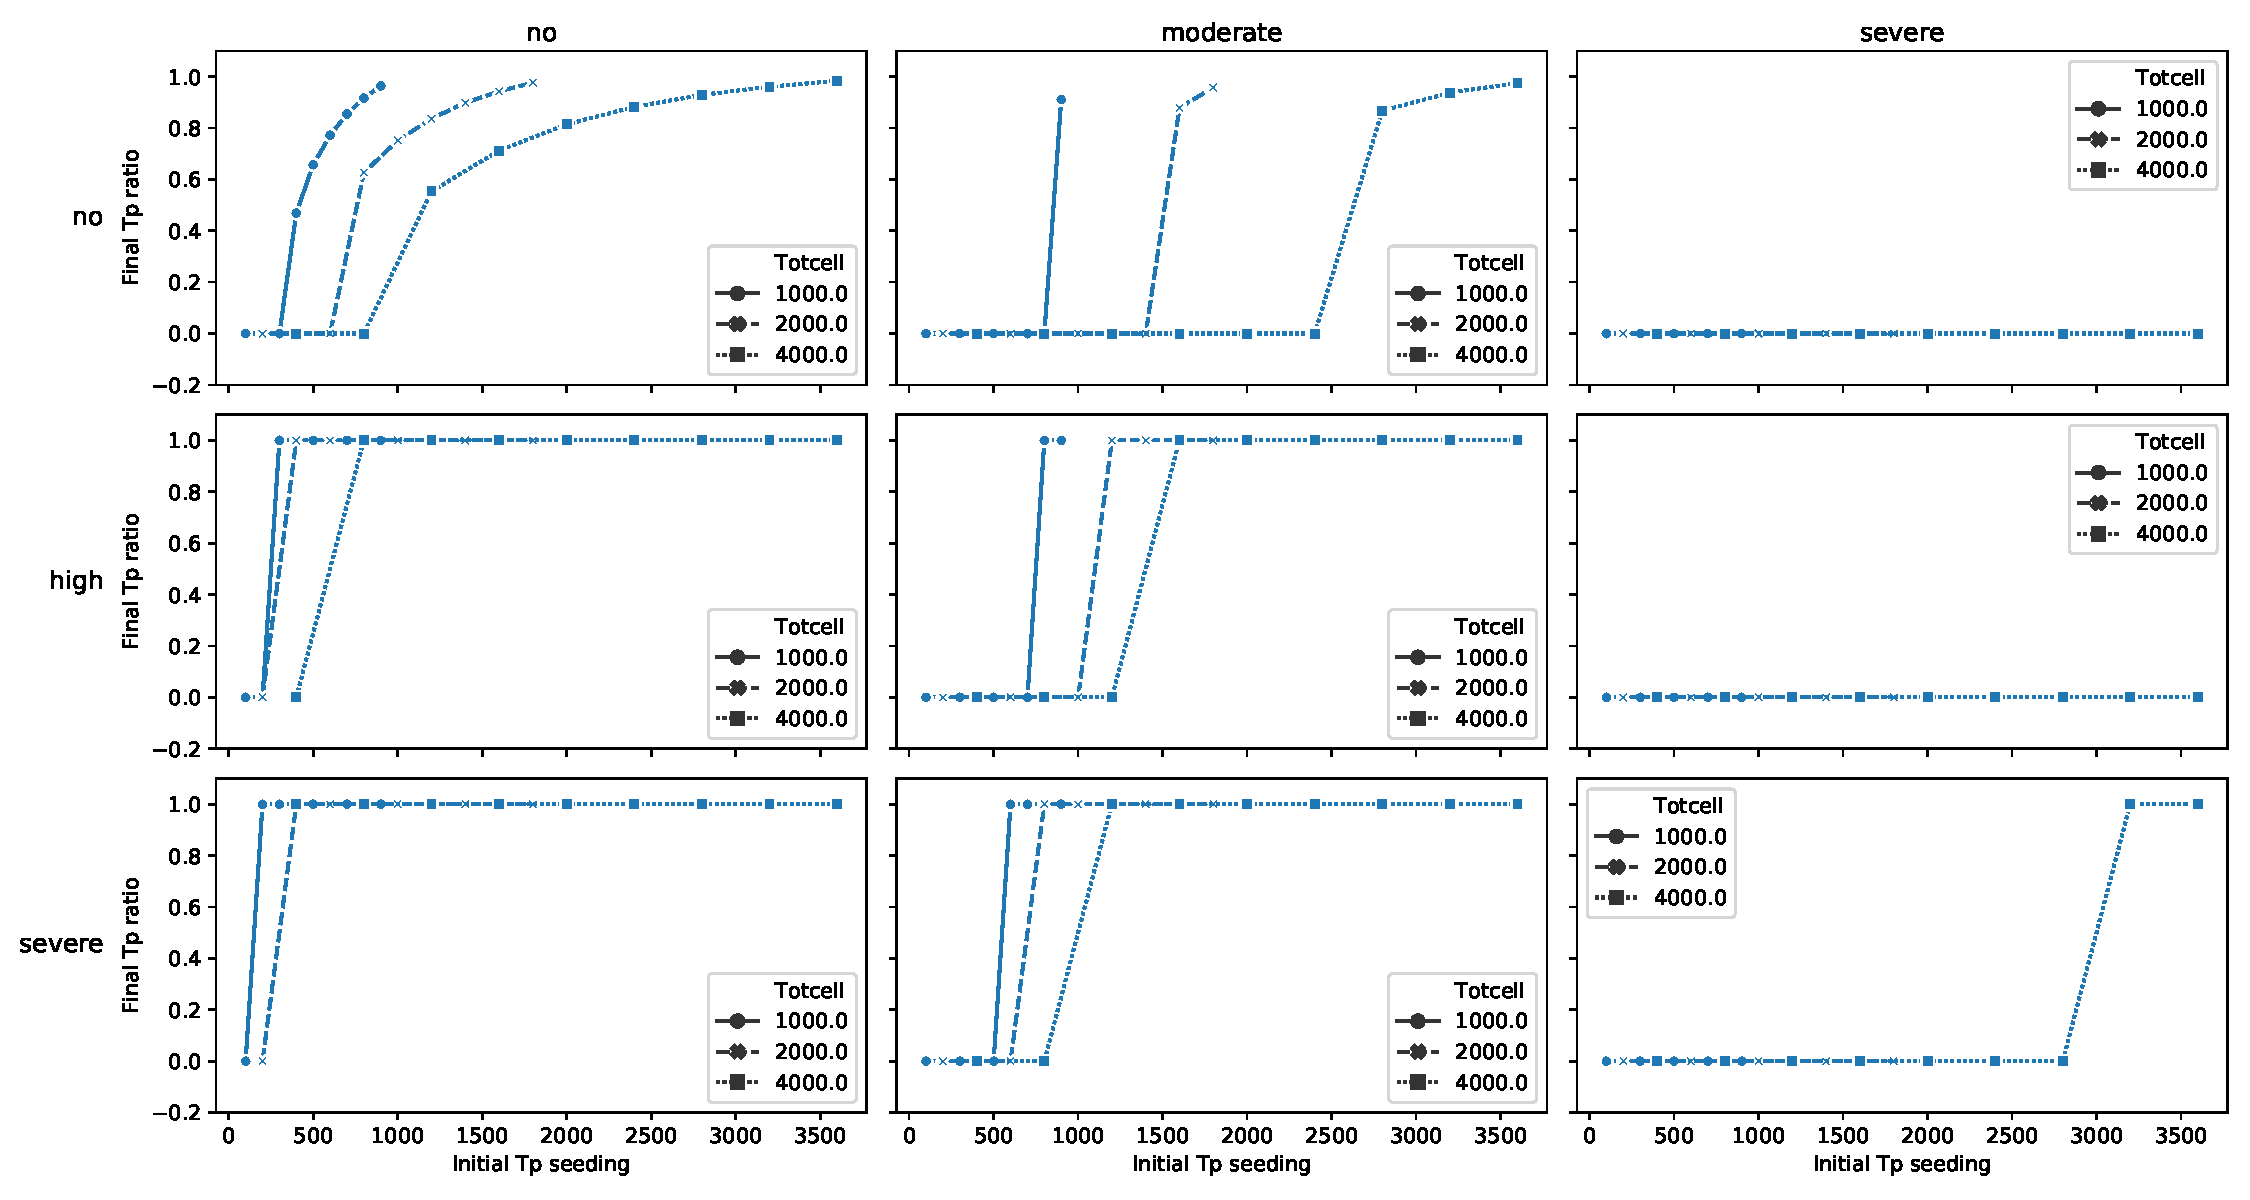
\includegraphics[width=\textwidth]{Tpro-Tneg_cases_normal}
      \caption{normal prodn.}
    \end{subfigure}
    \begin{subfigure}[b]{0.48\textwidth}
      \centering
      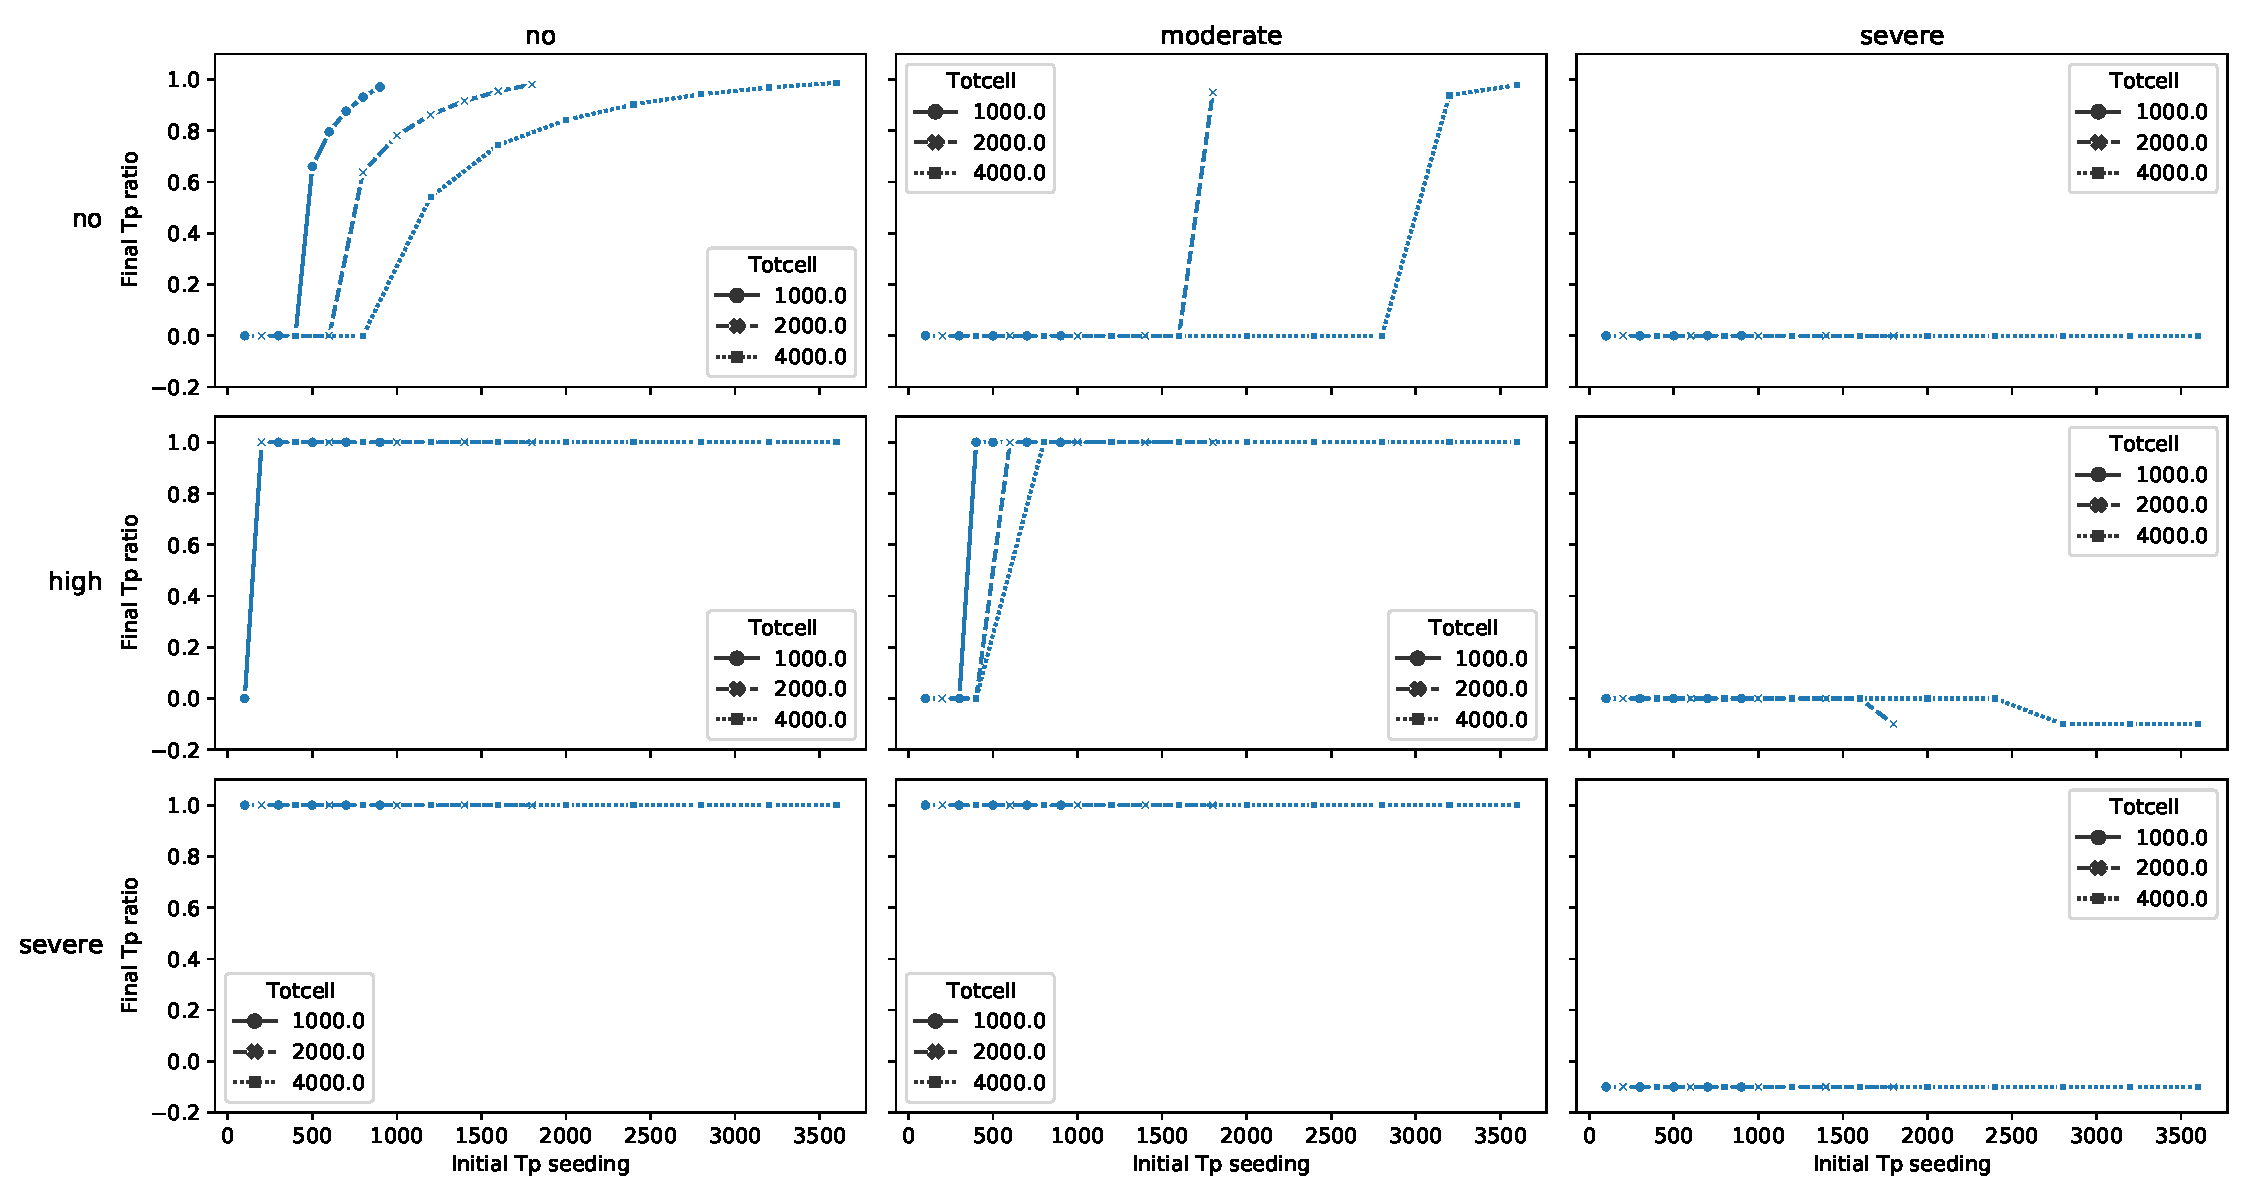
\includegraphics[width=\textwidth]{Tpro-Tneg_cases_poor}
      \caption{poor prodn.}
    \end{subfigure}
    \caption{Final $T^p$ ratio of pairwise $T^p - T^-$. SF: $O_2$ prodn., C: $T^p\ test$ limits, R: $T^-\ O_2$ limits.}
  \end{figure}
  \begin{columns}
    \begin{column}{0.5\textwidth}
      \begin{itemize}
        \item Coexist: $T^p$ no/mod. + $T^-$ low
      \end{itemize}
    \end{column}
    \begin{column}{0.5\textwidth}
      \begin{itemize}
        \item Tot. popn. vs Initial propn.
      \end{itemize}
    \end{column}
  \end{columns}
\end{frame}


\begin{frame}[allowframebreaks]{$T^+$ - $T^p$ Cases}
  \begin{figure}[h]
    \centering
    \begin{subfigure}[b]{0.48\textwidth}
      \centering
      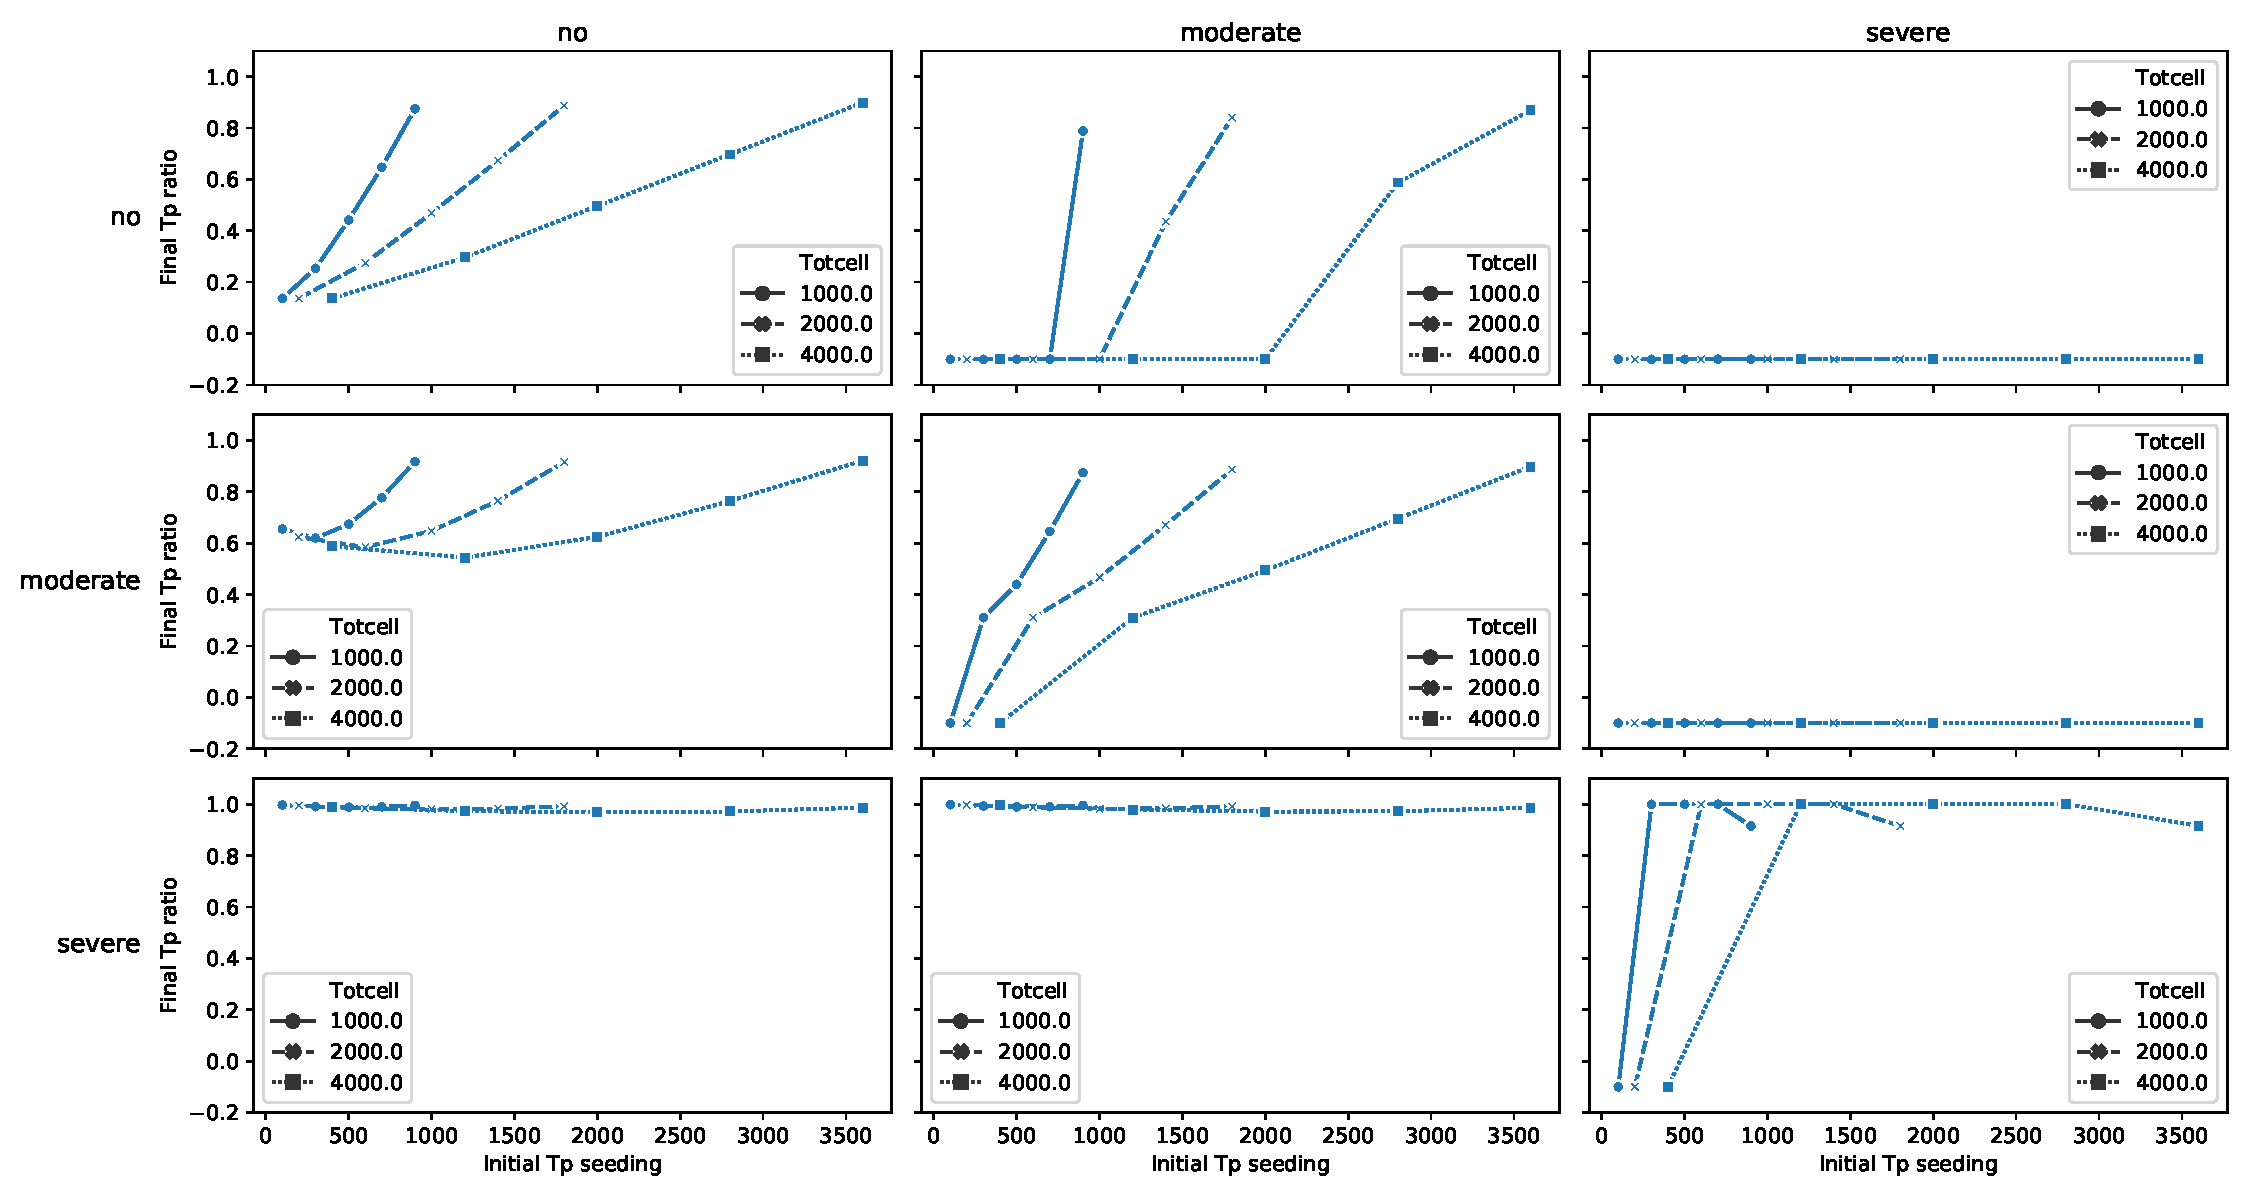
\includegraphics[width=\textwidth]{Tpos-Tpro_cases_test}
      \caption{$test$ limits. C: $T^p\ test$ limits, R: $T^+\ test$ limits}
    \end{subfigure}
    \begin{subfigure}[b]{0.48\textwidth}
      \centering
      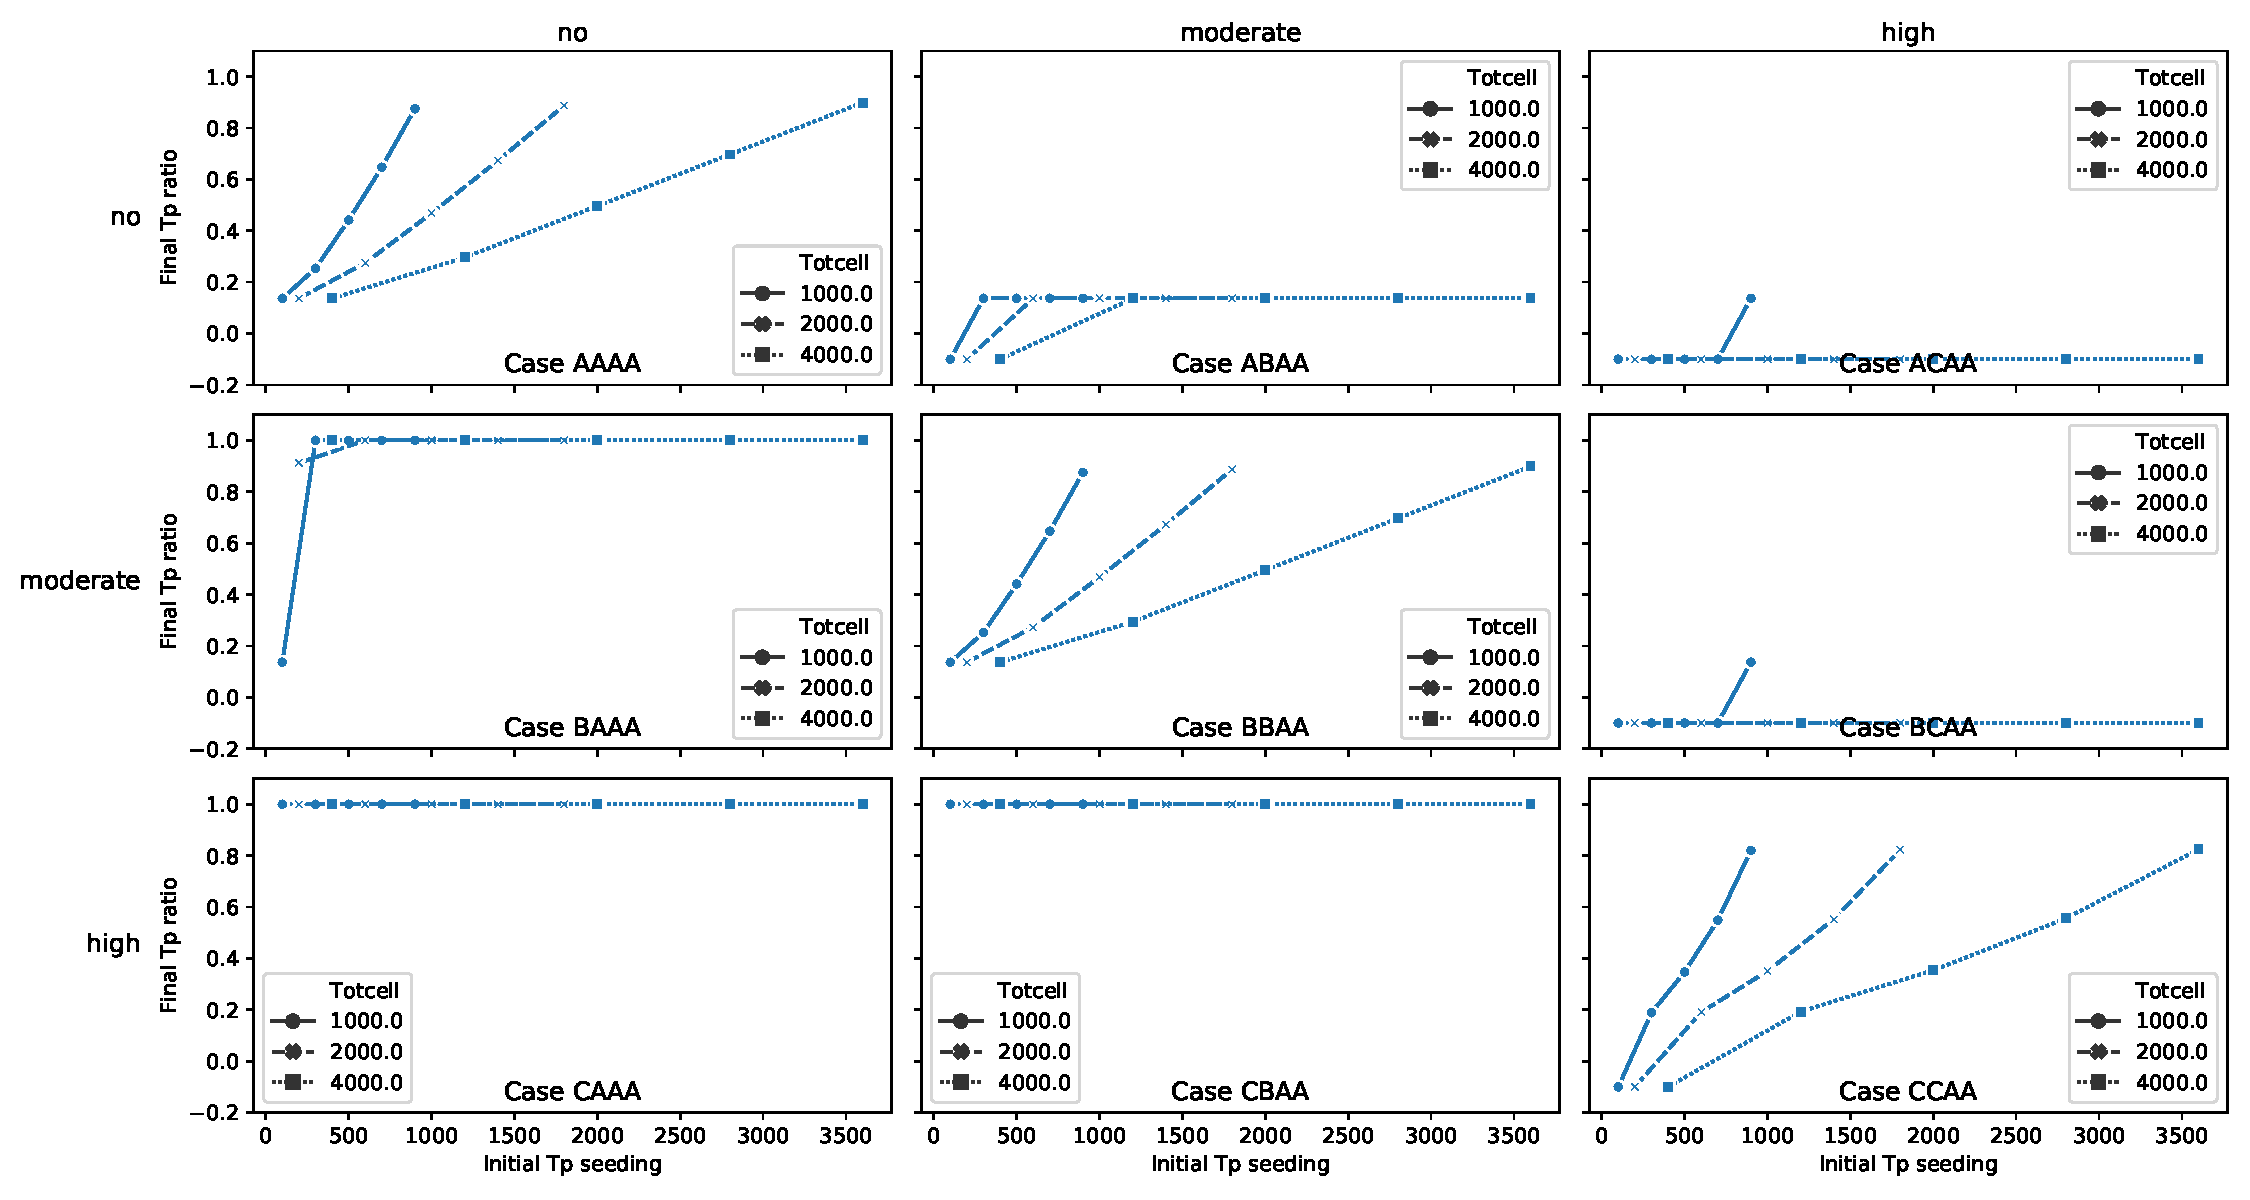
\includegraphics[width=\textwidth]{Tpos-Tpro_cases_o2}
      \caption{$O_2$ limits. C: $T^p\ O_2$ limits, R: $T^+\ O_2$ limits}
    \end{subfigure}
    \caption{Final $T^p$ ratio of pairwise $T^+ - T^p$}
  \end{figure}
  \begin{columns}
    \begin{column}{0.5\textwidth}
      \begin{itemize}
        \item Coexist: limitation same
      \end{itemize}
    \end{column}
    \begin{column}{0.5\textwidth}
      \begin{itemize}
        \item Coexist: mod.
      \end{itemize}
    \end{column}
  \end{columns}
  \framebreak
  \begin{figure}[h]\ContinuedFloat
    \centering
    \begin{subfigure}[b]{\textwidth}
      \centering
      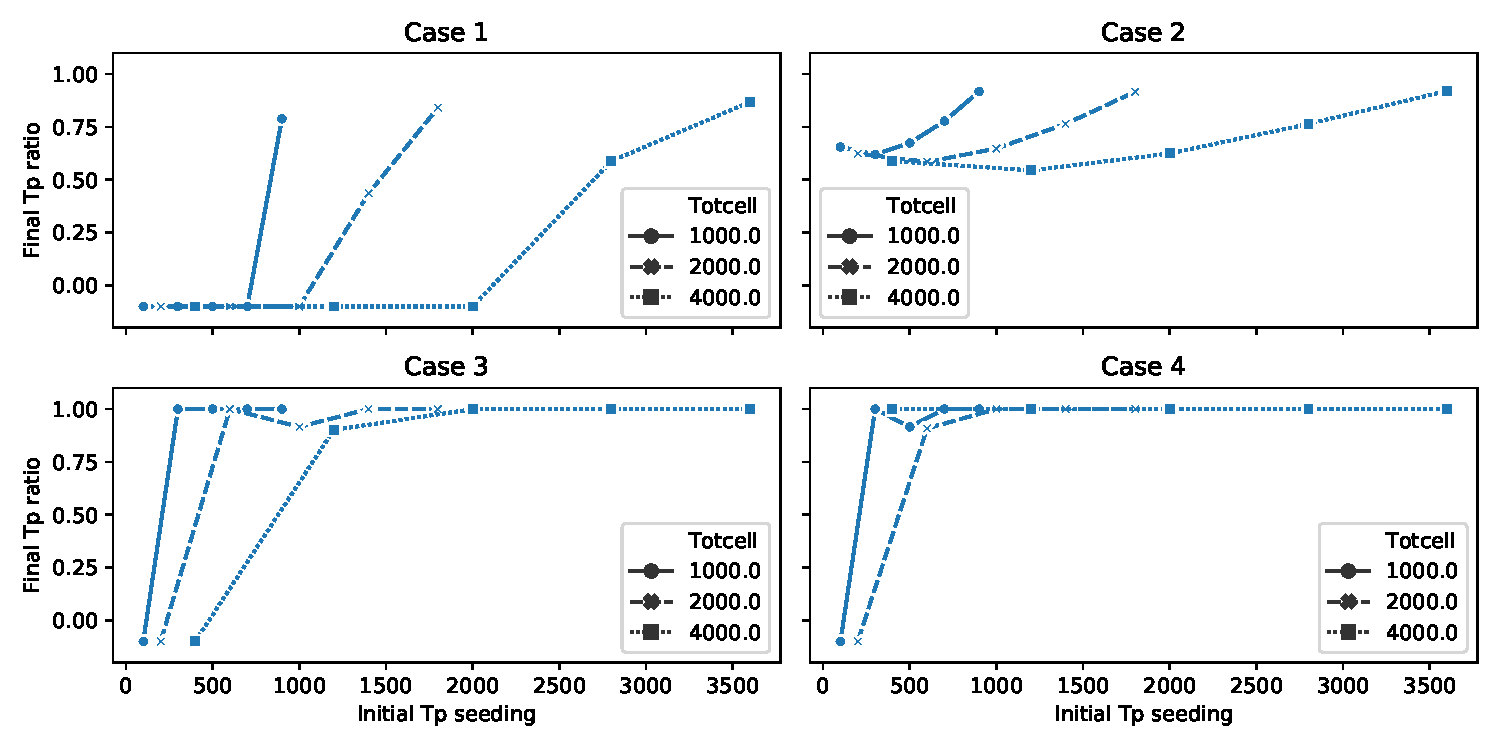
\includegraphics[width=0.5\textwidth]{Tpos-Tpro_cases}
      \caption{Combination limits. C: $T^+,T^p\ test$ limits, R: $T^+,T^p\ O_2$ limits}
    \end{subfigure}
    \caption{Final $T^p$ ratio of pairwise $T^+ - T^p$}
  \end{figure}
  \begin{itemize}
    \item Similar: symmetric limitation
  \end{itemize}
\end{frame}

\begin{frame}{All cell type cases}
  \begin{figure}[h]
    \centering
    \begin{subfigure}[b]{0.48\textwidth}
      \centering
      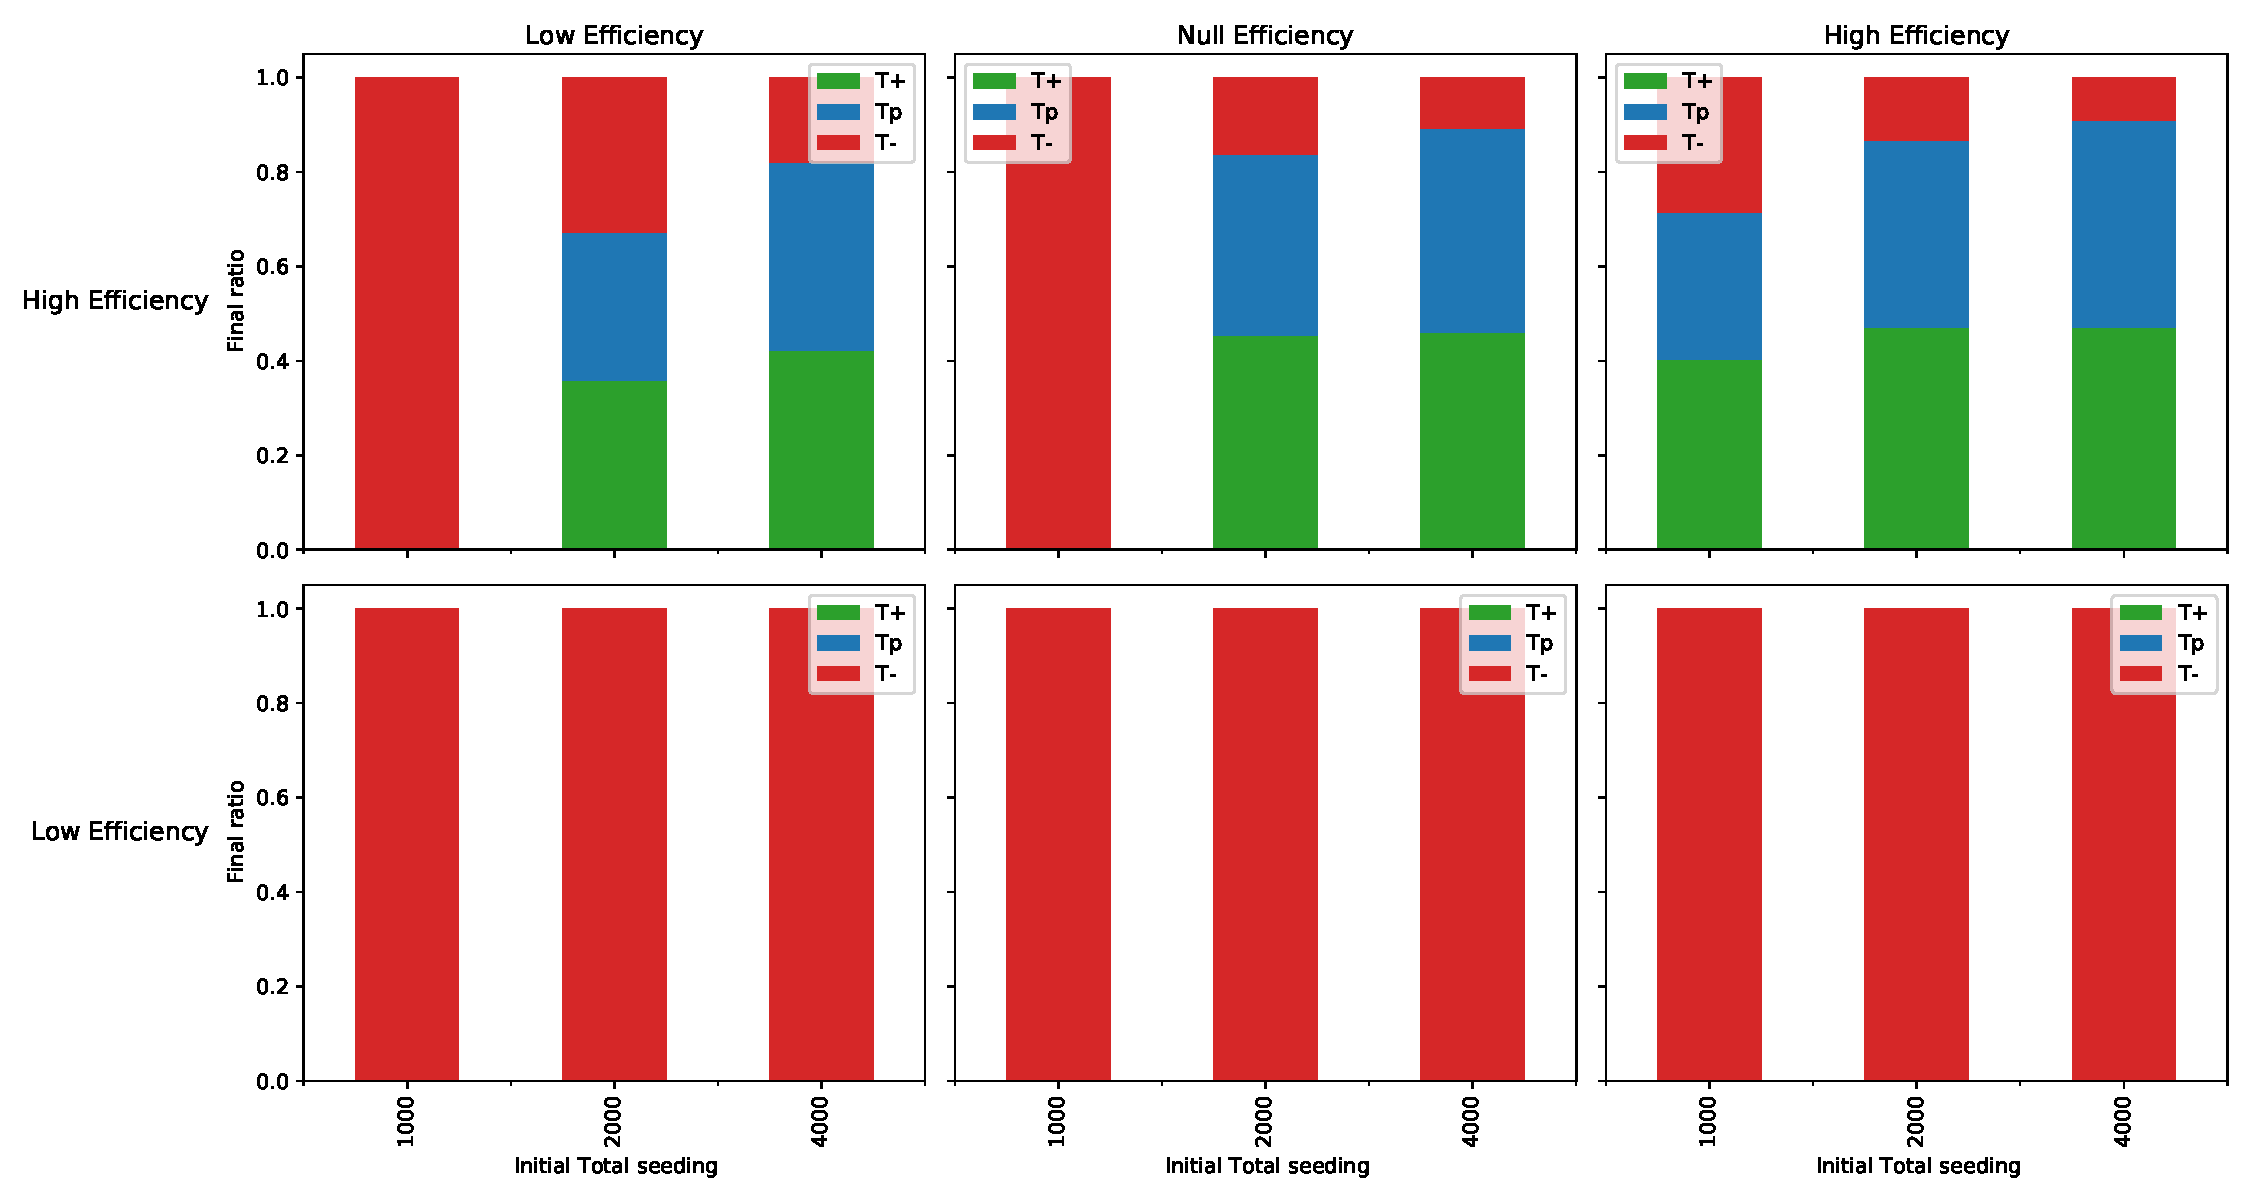
\includegraphics[width=\textwidth]{All3_efficiency_1:1:1}
      \caption{Equal seeding - 1:1:1 }
    \end{subfigure}
    \begin{subfigure}[b]{0.48\textwidth}
      \centering
      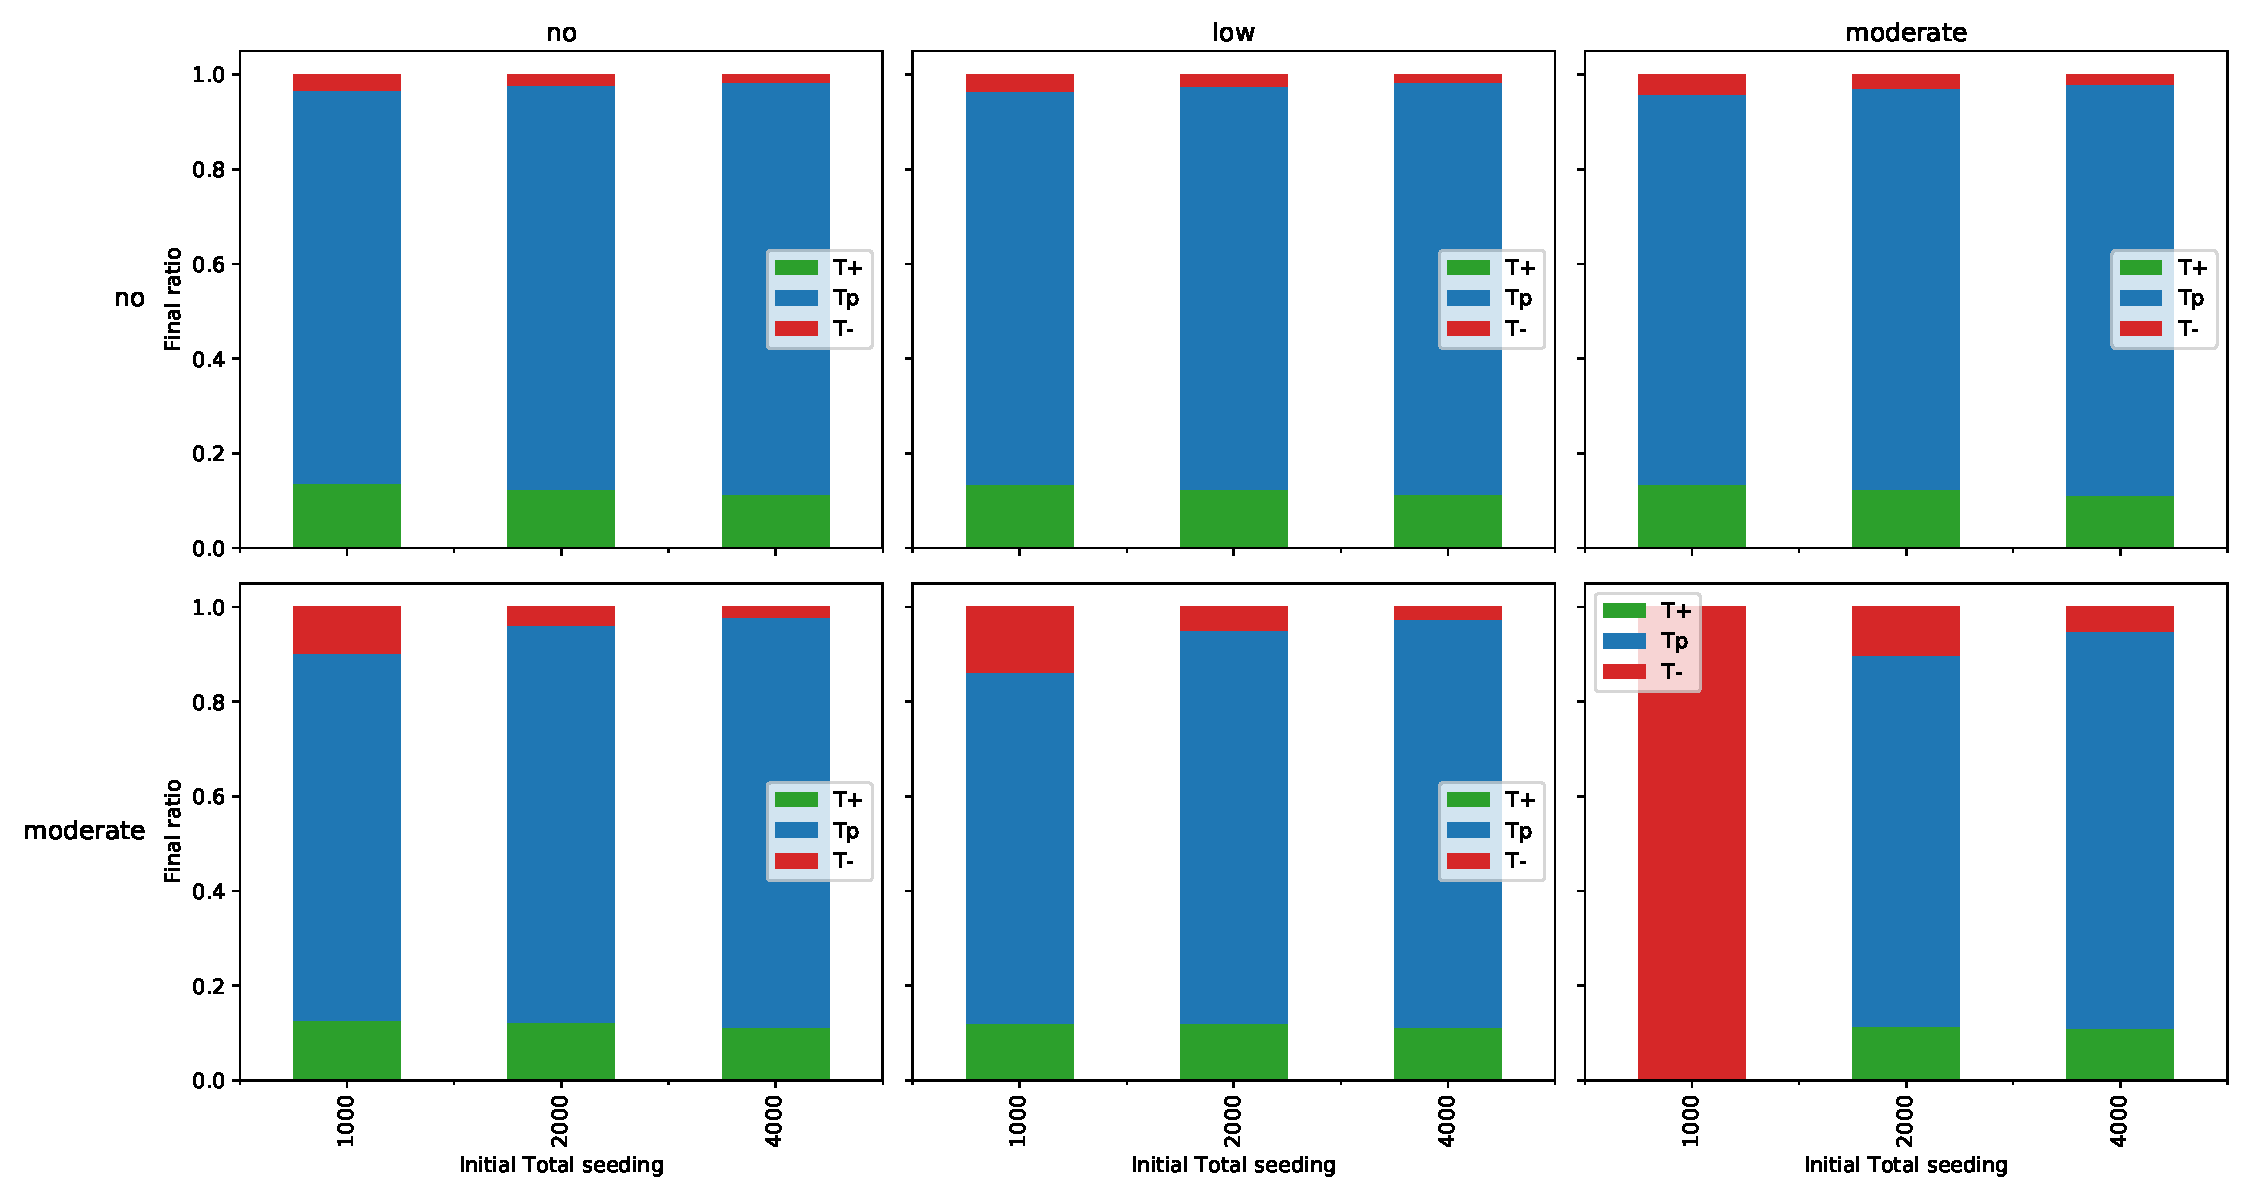
\includegraphics[width=\textwidth]{All3_efficiency_8:1:1}
      \caption{High $T^p$ seeding - 8:1:1}
    \end{subfigure}
    \caption{Final ratio of all cell types. C: $O_2$ limits , R: $test$ limits and SF: seeding propn.}
  \end{figure}
  \begin{columns}
    \begin{column}{0.5\textwidth}
      \begin{itemize}
        \item Homogenous: $test$ private resource
        \item No vs Mod: Weak vs Strong interspecific
      \end{itemize}
    \end{column}
    \begin{column}{0.5\textwidth}
      \begin{itemize}
        \item $O_2$: 3 zones of effect
      \end{itemize}
    \end{column}
  \end{columns}
\end{frame}
